\documentclass{article}
\usepackage[top=10mm, bottom=20mm, left=20mm, right=20mm]{geometry}
\usepackage{graphicx}

\parindent 0pt
\parskip 1em

\title{A Kinetic Perimetry Simulator in the OPI}
\author{Andrew Turpin, Astrid Zeman and Allison McKendrick}

\begin{document}
\maketitle

\section{Introduction}

Two key pieces of information allow us to use techniques for simulating static perimetric
responses for kinetic perimetric responses.

\begin{enumerate}

\item Phu et al. have shown that SKD (stato-kinetic dissociation) probably
does not exist for perimetric tasks, so it is reasonable to simulate responses to a
kinetic perimetric target based on simulated responses to static perimetric targets.

\item We have shown that the response time to kinetic targets follows a gamma distribution
just like response times to static targets.

\end{enumerate}

\section{Method}

We will determine the response to a kinetic vector by breaking it into a sequence of
static presentations, checking for static seen/not-seen at each of these 
until seen, and then adding a response time delay to get the final 
location of the response to return.
There is also allowance for a false positive or negative response.

Define a kinetic vector as the quintuple $(b,e,s,g,d)$, where
\begin{description}
    \item[$b$] is the $(x,y)$ coordinate of the beginning of the kinetic vector;
    \item[$e$] is the $(x,y)$ coordinate of the end of the kinetic vector;
    \item[$s$] is the speed of the target in degrees per second; 
    \item[$g$] is the Goldmann size of the target; and 
    \item[$d$] is the dB level of the target.
\end{description}


Define the probability of seeing a static target of $d$ dB given 
the true threshold is $t$ dB as 
$$
    p(d, t) = 1 - \Phi(d, \mu=t, \sigma=\min(6, e^{At + B})) 
$$
where $A$ and $B$ are the usual Henson et al. constants chosen appropriately for stimulus
size $g$, and $\Phi$ is the cummulative Gaussian distribution.

If we break the kinetic vector $\vec{be}$ into $n$ 
locations $\{b=(x_1,y_1),\ldots,(x_n,y_n)=e\}$ with the true static threshold at each location
being $\{t_1,\ldots,t_n\}$ respectively, then the probability of seeing the vector at
location $\ell \in[1,n]$ is 
$$
    P(\ell) = p(d, t_\ell) \prod_{i=1}^{\ell-1} (1 - p(d, t_i));
$$
that is, the product of the probability of seeing the static target at location $\ell$
and the probabilities of not seeing it at all previous locations $[1,\ell-1]$.
Obviously $P(1) = p(d,t_1)$.

\subsection{Response time adjustment}

Assuming that the stimuls is ``seen'' at location $(x_\ell,y_\ell)$ 
(that is, a random uniform number is $\le P(\ell)$), 
then a random amount along the path of the vector is added to get the final response
location.
The location to return is computed as 
\begin{eqnarray*}
x & = & x_\ell + (\tau\times s/1000) \cos(\theta) \\
y & = & y_\ell + (\tau\times s/1000) \sin(\theta) \\
\end{eqnarray*}
where $\tau$ is a response time in ms drawn from some gamma distribution that models the
patient's response time, 
and $\theta$ is the angle of the vector. Recall $s$ is the speed in degrees per second.


\subsection{False responses}

If the probability of a false positive response on any given trial is $f_p$, and a false
negative $f_n$, then we first toss a coin to see which to check for first. (If you always
check for one before the other, then the probability of the second occurring is decreased.)

False negatives occur when a random uniform number is less than $f_n$, and simply result 
in a not-seen response, and so are easily dealt with.

If a false positive occurs (uniform random is less than $f_p$), then we need to chose a
location along the vector where that false positive occurs. This is chosen randomly from
$\{\ell | P(\ell) \le 0, \ell\in[1,n]\}$, the set of 
any of the $n$ locations that have a probability of being seen of zero or less.


\section{Results}

\begin{figure}
  \centering
  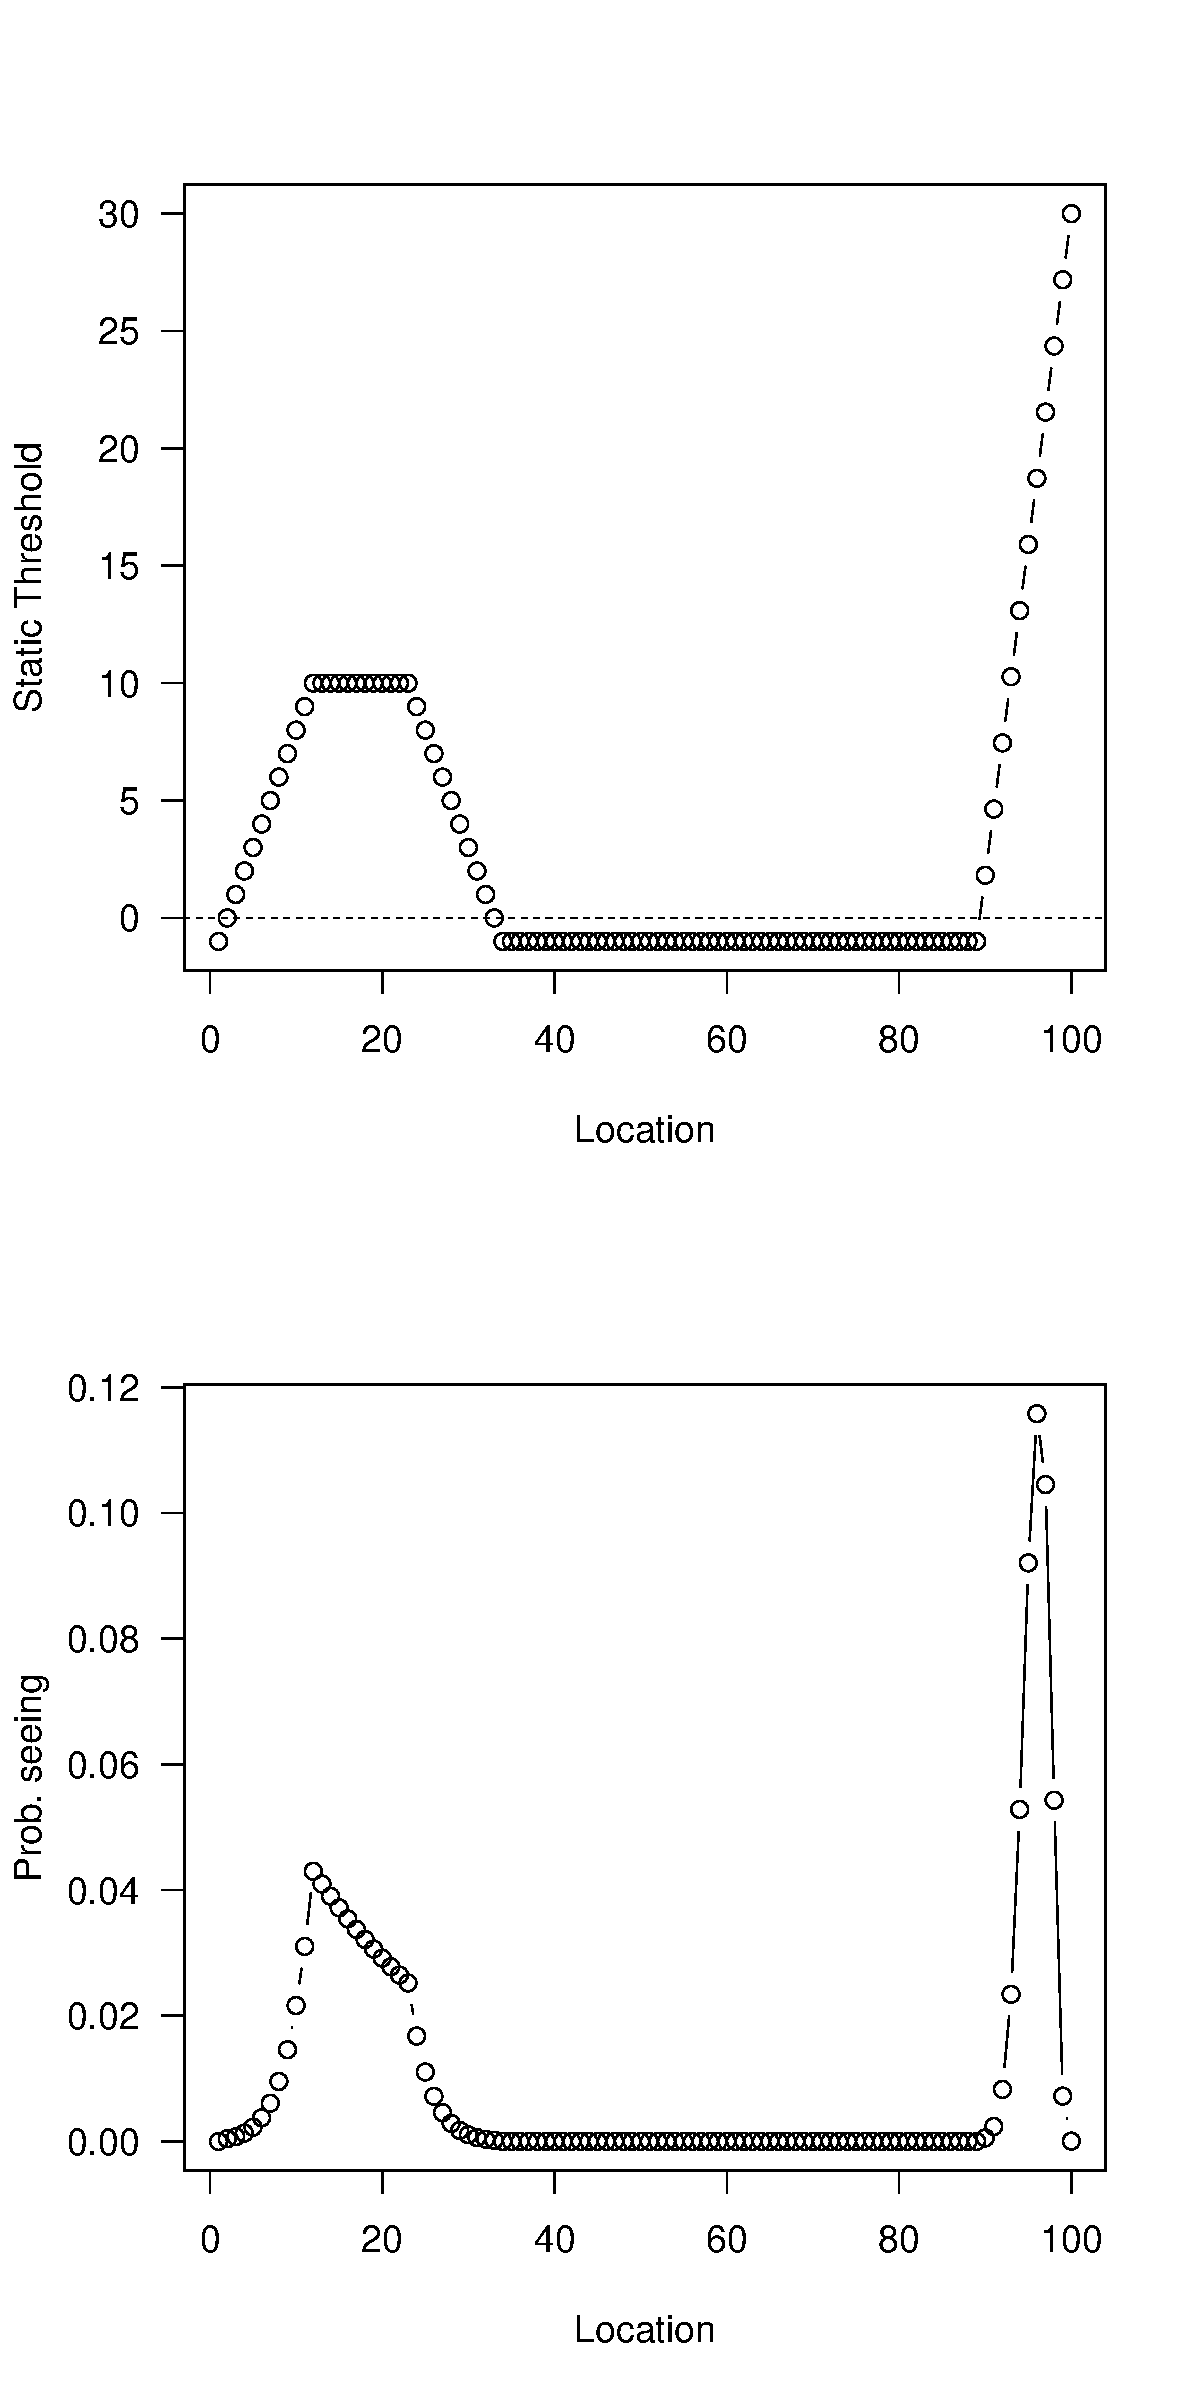
\includegraphics[scale=0.3,page=1]{eg1.pdf}
  \caption{Top panel shows true threshold input to kinetic simulator for a vector from 
        $(60,60)$ to $(0,0)$ broken into 100 steps. A threshold of -1 indicates never seen.
         The bottom panel shows $P$, the probability of 
         seeing the kinetic stimuli at location,
         assuming a Goldmann Size III stimulus at 25dB.
  }
  \label{fig-eg1}
\end{figure}


\end{document}

